%-----------------------------------------------------------------
%	DATA: ON DEVELOPING SYSTEMS
%	!TEX root = ./../main.tex
%-----------------------------------------------------------------
% \newpage
\subsection{On non-developing systems}
% As we mentioned in~\cref{sec:pdi-vs-sst}, we want to find a correlation between the $PDI$ and the duration of the storms, or their wind speeds. Instead of using the whole tropical-cyclones data set as is, we will separate developing from non-developing systems.
Tropical-cyclones that surpass the $\SI{33}{\knot}$ wind speed threshold are called \emph{developing systems}, while the ones that do not do so are called \emph{non-developing systems}. In terms of hydrodynamics, the major difference between developing and non-developing systems is that the developing have a distinct area of low height or low pressure centred on the system, i.e., they form cyclones~\cite{McBride1979}.

This means that even though all tropical-cyclones behave thermodynamically in the same way throughout their lifetime (the $PDI$ calculation is valid for all their life span), the wind speeds evolve rather differently depending on the development status of the storm.

% For this reason, one should play on the cautious side and study developing and non-developing systems separately, as they represent different physical systems.

\medskip
% \todo[inline]{NON-STATIONARY}
Apart from this physical description, from a statistical point of view, one can see that non-developing systems constitute a \emph{nonstationary} time series for the North Atlantic data (\Cref{fig:natl-storms-ts} and \Cref{tab:natl-storms-ts-stationarity}); this means the distribution of the storms alters with alterations in time.

% \todo{Expand this paragraph}
\begin{figure}[H]
	\centering
	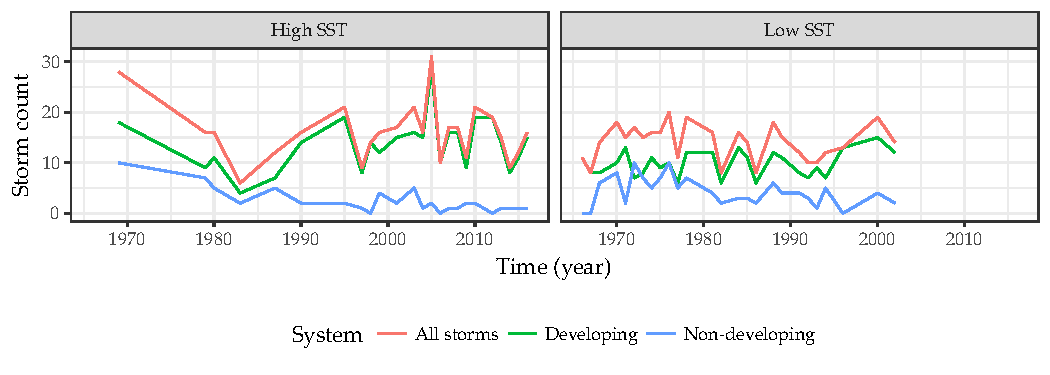
\includegraphics[width=\textwidth]{images/natl-storms-ts}
	\caption{Time series of storm occurrences for the North Atlantic basin, emphasising into non-developing systems and developing systems}
	\label{fig:natl-storms-ts}
\end{figure}

\begin{table}[H]
	\centering
	\begin{tabular}{lccc}
		\toprule
		\toprule
		Subset     & Non-developing & Developing & All storms \\
		\midrule
		All storms &  $0.0205$      & $\geq 0.1$ & $\geq 0.1$ \\
		Low SST    &  $0.0233$      & $\geq 0.1$ & $\geq 0.1$ \\
		High SST   &  $0.0429$      & $\geq 0.1$ & $\geq 0.1$ \\
		\bottomrule
		\bottomrule
	\end{tabular}
	\caption{List of $p$-values associated with the Kwiatkowski--Phillips--Schmidt--Shin test to analyse stationarity of the storm occurrences for the North Atlantic basin}
	\label{tab:natl-storms-ts-stationarity}
\end{table}

For the Northeast Pacific data (\Cref{fig:epac-storms-ts} and \Cref{tab:epac-storms-ts-stationarity}), stationarity is rejected only for the time series without separation of the storms by SST class.

\begin{figure}[H]
	\centering
	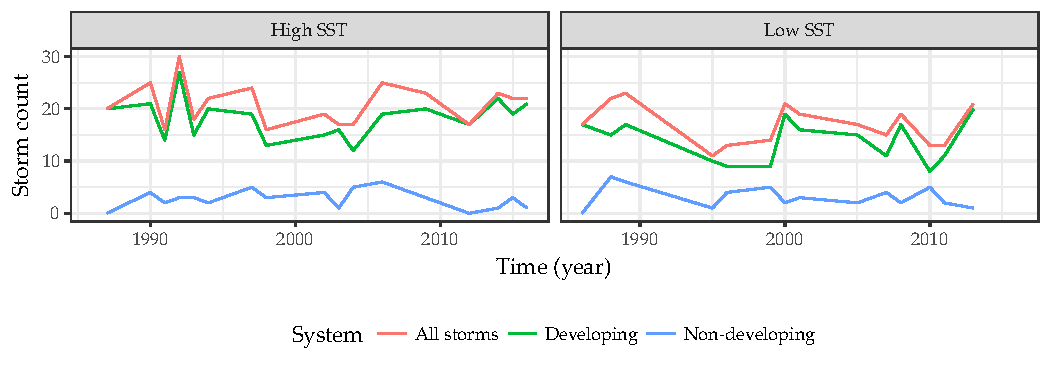
\includegraphics[width=\textwidth]{images/epac-storms-ts}
	\caption{Time series of storm occurrences for the Northeast Pacific basin, emphasising into non-developing systems and developing systems}
	\label{fig:epac-storms-ts}
\end{figure}

\begin{table}[H]
	\centering
	\begin{tabular}{lccc}
		\toprule
		\toprule
		Subset     & Non-developing & Developing & All storms \\
		\midrule
		All storms &  $0.0294$      & $\geq 0.1$ & $\geq 0.1$ \\
		Low SST    &  $0.0732$      & $\geq 0.1$ & $\geq 0.1$ \\
		High SST   &  $0.0733$      & $\geq 0.1$ & $\geq 0.1$ \\
		\bottomrule
		\bottomrule
	\end{tabular}
	\caption{List of $p$-values associated with the Kwiatkowski--Phillips--Schmidt--Shin test to analyse stationarity of the storm occurrences for the Northeast Pacific basin}
	\label{tab:epac-storms-ts-stationarity}
\end{table}

The issue with this is that when nonstationary time series are used in a regression model one may obtain apparently significant relationships from unrelated variables. This phenomenon is called \emph{spurious regression}~\cite{Phillips1986}. For example, if the series is consistently increasing over time, the sample mean and variance will grow with the size of the sample, and they will always underestimate the mean and variance in future periods. And if the mean and variance of a series are not well-defined, then neither are its correlations with other variables.

One should be cautious, therefore, about trying to extrapolate regression models fitted to nonstationary data.

\bigskip
Although we do not perform a direct regression analysis on the time series of storm occurrences, our data is temporally distributed following this time series. Thus, to be on the cautious side, as they represent different physical systems and may introduce problems in the regression analysis, for our study, we opt to exclude non-developing systems altogether.

One could argue that this is not necessary for the Northeast Pacific basin, but to be consistent in the methodology applied to both basins, we exclude non-developing systems as well.
